\documentclass[main]{subfiles}
\usepackage{graphicx}

\begin{document}

\chapter{Task description of the VPW}\label{ch:task-description-of-the-flemisch-programming-contest}

{
\itshape Below is a translated version of the second Scratch exercise from the 2017 edition of the Flemish Programming Contest (\textdutch{Vlaamse Programmeerwedstrijd}, \textsc{VPW}).
Afterwards, one potential solution is shown.
}

\fbox{%
    \begin{minipage}{\textwidth}
        \minisec{Problem 02 (10 points)}
        The stage looks like the drawing below.

        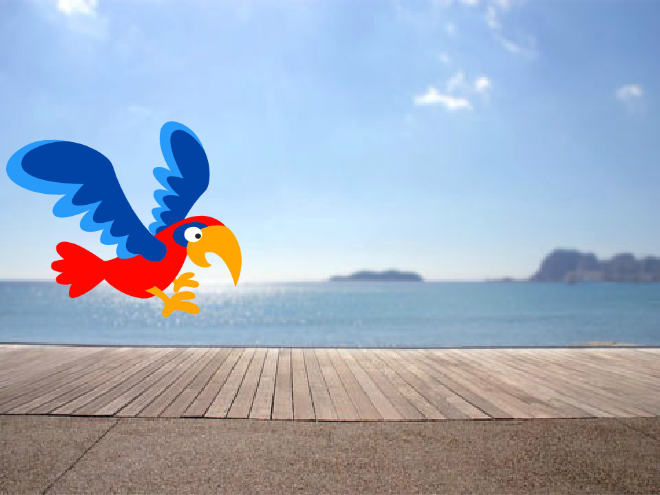
\includegraphics[width=0.5\textwidth]{stage-02}

        Write a program that lets the parrot fly from left to right.
        When he touches the edge, he must turn around.
        The program may only start when the parrot is clicked.
        (Tip: use the ``change costume to \dots'' block for flying)
    \end{minipage}
}

\begin{center}
    \begin{varwidth}{0.6\textwidth}
        \begin{scratch}[scale=0.6]
            \blockinit{when this sprite clicked}
            \blockmove{set rotation style \selectmenu{left-right}}
            \blockinfloop{forever}{
                \blockmove{move \ovalnum{15} steps}
                \blockmove{if on edge, bounce}
            }
        \end{scratch}
    \end{varwidth}%
    \hspace{1em}%
    \begin{varwidth}{0.6\textwidth}
        \begin{scratch}[scale=0.6]
            \blockinit{when this sprite clicked}
            \blockinfloop{forever}{
                \blockevent{wait \ovalnum{0.2} seconds}
                \blocklook{next costume}
            }
        \end{scratch}
    \end{varwidth}
\end{center}


\end{document}
